 \documentclass[12pt,a4paper]{article}
\usepackage{pgfplots}
\usepackage{tikz}
\usetikzlibrary{backgrounds}
\usepackage{import}
\usepackage[font=scriptsize,labelfont=bf]{caption}
\usepackage{float}

\begin{document}

\newcommand*{\figuretitle}[1]{%
    {\centering%   <--------  will only affect the title because of the grouping (by the
    \textbf{#1}%              braces before \centering and behind \medskip). If you remove
    \par\medskip}%            these braces the whole body of a {figure} env will be centered.
}


\section{ensembl with 8880 genes families and 15 species}

\subsection{Parallel efficiency  (reference: 32 cores)}

In a perfect world, this should be an horizontal line

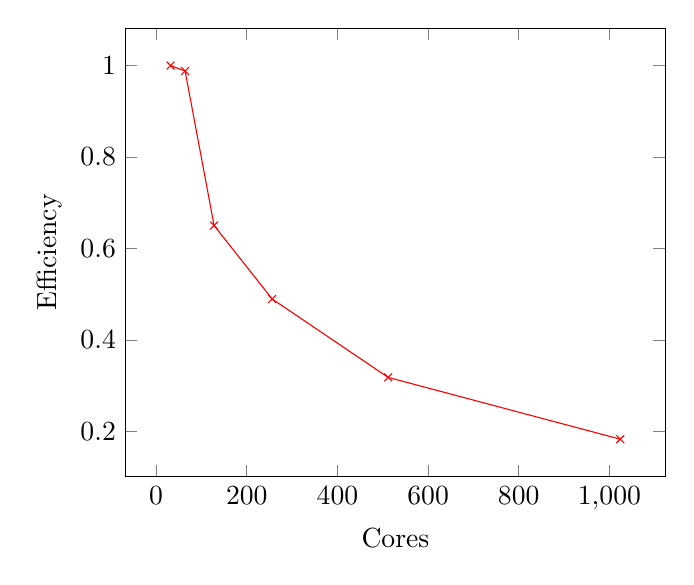
\begin{tikzpicture} 
\begin{axis}[ xlabel=Cores, ylabel=Efficiency] 
	\addplot[color=red,mark=x] 
		coordinates { (32, {(51518 * 32)/(51518 * 32)}) (64, {(51518 * 32)/(26070 * 64)}) (128,{(51518 * 32)/(19813 * 128)}) (256,{(51518 * 32)/(13157*256)}) (512,{(51518 * 32)/(10127*512)}) (1024, {(51518 * 32)/(8806*1024))}) }; 
\end{axis} 
\end{tikzpicture}

\subsection{Runtime per core}

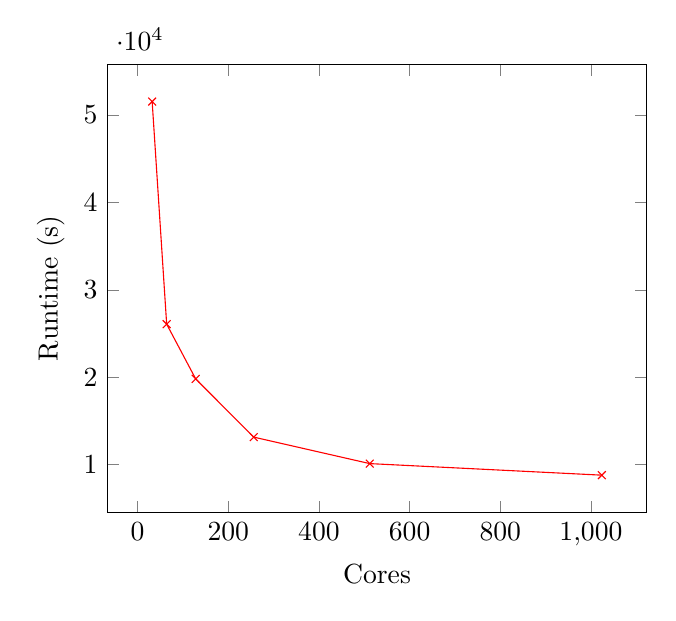
\begin{tikzpicture} 
\begin{axis}[ xlabel=Cores, ylabel=Runtime (s)] 
	\addplot[color=red,mark=x] 
		coordinates {  (32, 51518) (64, 26070) (128,19813) (256,13157) (512,10127) (1024, 8806) }; 
\end{axis} 
\end{tikzpicture}


\end{document}